\documentclass[preview]{standalone}
%\usepackage{geometry}
%graphics
\usepackage{xcolor}
\usepackage{tikz}
\usetikzlibrary{shapes.geometric, shapes.multipart, arrows, calc, through}
\usepackage[caption=false,font=footnotesize]{subfig}

\colorlet{dot-color}{black!80}
\tikzset{
    pics/block/.style = {
        code = {%
        \fill[gray]  (-1.6,-1.3)  rectangle (1.6,1.3);
        \fill[white] (0.2,0.1)   rectangle (1.4,1.1);
        \fill[white] (-1.4,0.1)  rectangle (-0.2,1.1);
        \fill[white] (0.2,-1.1)  rectangle (1.4,-0.1);
        \fill[white] (-1.4,-1.1) rectangle (-0.2,-0.1);
        \fill[{black!70}] (-0.5,-0.5) rectangle (0.5,0.5);
        }
    },
    pics/pad/.style = {
        code = {%
            \draw[fill=white] (-0.05,0) -- (-0.05,0.5) -- (-0.25,0.5) -- (-0.25,1) -- (0.25,1) -- (0.25,0.5) -- (0.05,0.5) -- (0.05,0) -- cycle;
        }
    },
}

\begin{document}

\begin{figure}[!t]
\centering
\subfloat[]{
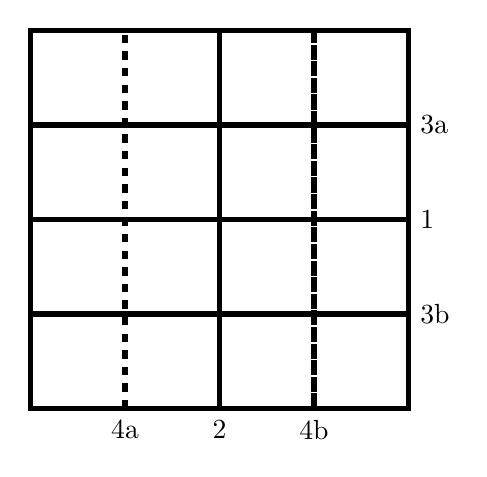
\begin{tikzpicture}[line width=2pt, scale=0.6]
\draw (-4,-4) rectangle (4,4);
\draw (-4,0) rectangle (4,0) node[right]{1};
\draw (0,-4)node[below]{2} rectangle (0,4);
\draw (-4,2) rectangle (4,2) node[right]{3a};
\draw (-4,-2) rectangle (4,-2) node[right]{3b};
\draw[dashed] (-2,-4)node[below]{4a} rectangle (2,4);
\draw[dashed] (2,-4)node[below]{4b} rectangle (2,4);

\end{tikzpicture}
}
\hfil
\subfloat[]{
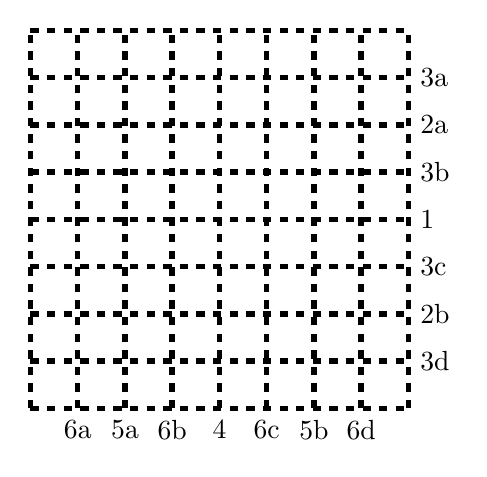
\begin{tikzpicture}[line width=2pt, scale=0.6]
\draw[step=1, dashed] (-4,-4) grid (4,4); 
\node[right] at(4,0) {1};
\node[right] at(4,2) {2a};
\node[right] at(4,-2) {2b};
\node[right] at(4,3) {3a};
\node[right] at(4,1) {3b};
\node[right] at(4,-1) {3c};
\node[right] at(4,-3) {3d};

\node[below] at(0,-4){4};
\node[below] at(-2,-4){5a};
\node[below] at(2,-4){5b};
\node[below] at(-3,-4){6a};
\node[below] at(-1,-4){6b};
\node[below] at(1,-4){6c};
\node[below] at(3,-4){6d};
\end{tikzpicture}
}
\end{figure}

\end{document}
